\documentclass{beamer}
\usetheme{metropolis}           % Use metropolis theme
\usepackage{appendixnumberbeamer}
\usepackage{epigraph}
\usepackage{color}
\usepackage{amsopn}
\usepackage{framed}             % for {framed}
\usepackage{tabto}
\graphicspath{{../img/}}
\usepackage{skak}           % for typesetting Chess

\theoremstyle{definition}
\newtheorem{defn}{Definition}

%%% Bibliography
\usepackage[backend=bibtex, style=authoryear]{biblatex}
\AtBeginBibliography{\tiny}
\bibliography{../src/bibliography.bib}

\setbeamercolor{background canvas}{bg=white}
\setbeamercolor{title}{fg=white}
\setbeamercolor{author}{fg=white}
\setbeamercolor{date}{fg=gray}
\setbeamercolor{institute}{fg=gray}

\newcommand{\todo}{\alert{TODO}}
\newcommand{\itemBullet}{\scriptsize$\blacksquare$}
\setbeamertemplate{itemize item}{\itemBullet}
\setbeamertemplate{itemize subitem}{\itemBullet}
\setbeamertemplate{itemize subsubitem}{\itemBullet}
\newcommand{\E}{\mathop{\mathbb{E}}}
\DeclareMathOperator*{\argmax}{arg\,max}
\newcommand{\epiParSpace}{\vskip 1.5ex}
\newcommand{\vect}[1]{\boldsymbol{#1}}
\newcommand{\I}{\mathcal{I}}
\newcommand{\dt}{\tilde{d}}
\newcommand{\It}{\tilde{I}}
\newcommand{\cfrplus}{CFR\textsuperscript{+}~}

\title{Solving Endgames \\in~Large Imperfect-Information Games \\such as~Poker}
\date{September 13, 2016}
\author{Bc.~Karel Ha}
\institute{Department of~Applied Mathematics \\Charles University}

\begin{document}
  {
    \usebackgroundtemplate{
      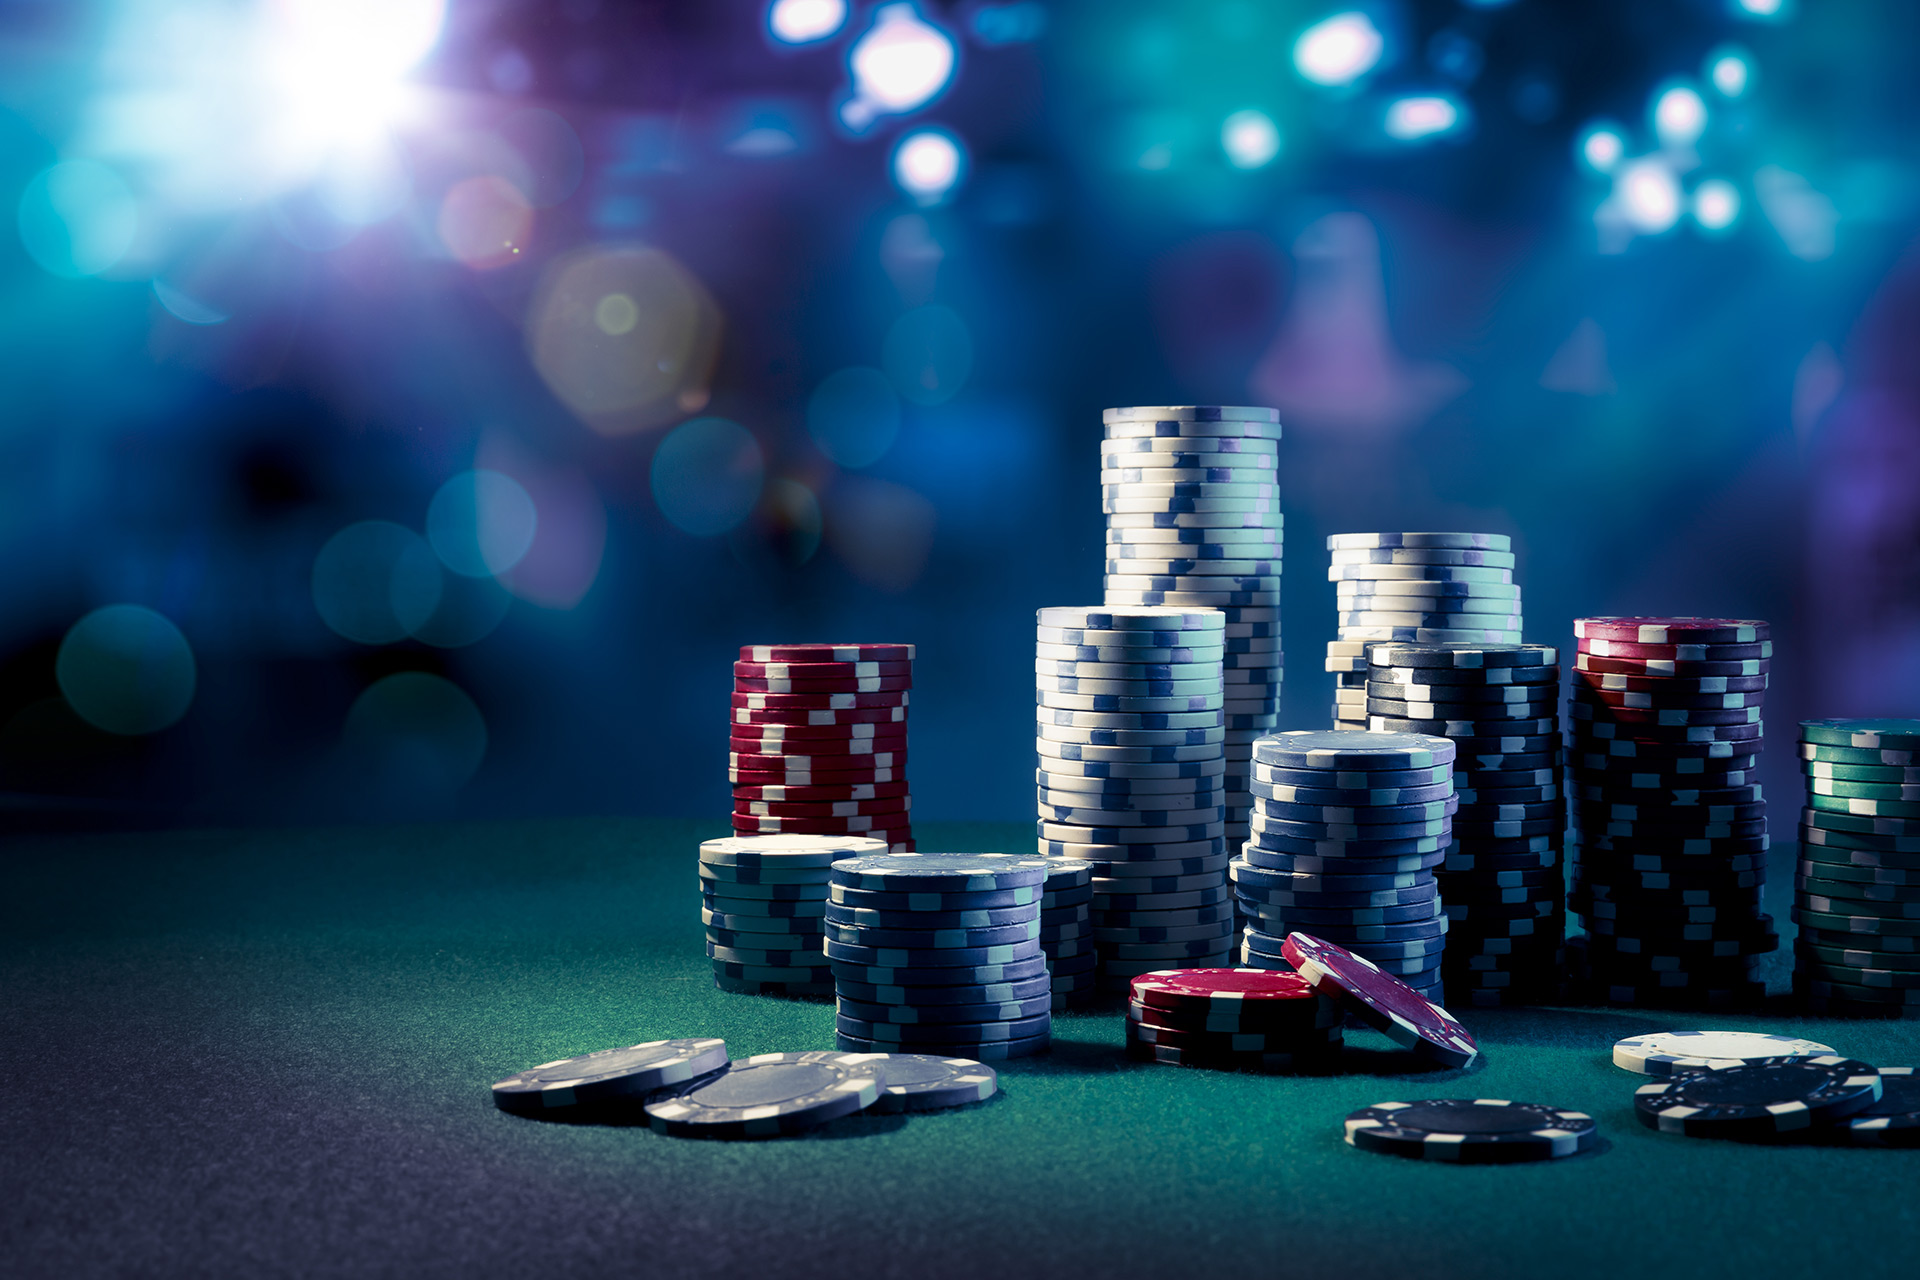
\includegraphics[height=\paperheight]{../img/poker_bg.jpg}
    }
    \maketitle
  }

  \section{Perfect-Information Subgames}

  \begin{frame}{Perfect-Information Subgames: Subgame / Endgame}
    Any node in~the tree induces its own subgame:
    \pause
    \begin{figure}[H]
      \raggedleft
      \scriptsize
      \def\svgwidth{.8\textwidth}
      \input{../img/extended-form_subgame.pdf_tex}
    \end{figure}
  \end{frame}

  \begin{frame}{Endgames in Classic Games}
    \pause
    \begin{itemize}[<+- | alert@+>]
      \item Go
        \begin{itemize}
          \item combinatorial game theory
          \item simulations: Monte Carlo tree search + neural networks
        \end{itemize}
      \item Chess
        \begin{itemize}
          \item retrograde analysis (backward induction)
        \end{itemize}
    \end{itemize}
  \end{frame}

  {
    \setbeamertemplate{frame footer}{\cite{Lomonosov2014eightlongest}}
    \def\chessTitle{Chess Endgames: Longest 7-man Checkmate }
    \begin{frame}{\chessTitle (549 Moves)}
      \begin{figure}[H]
        \centering
        \newgame
        \fenboard{1n1k4/6Q1/5KP1/8/7b/1r6/8/8 w - - 0 0}
        \showboard
      \end{figure}
    \end{frame}

    \begin{frame}{\chessTitle (549 Moves)}
      \begin{figure}[H]
        \centering
        \fenboard{1n1k4/6Q1/6P1/5K2/7b/1r6/8/8 b - - 0 0}
        \showboard
      \end{figure}
    \end{frame}

    \begin{frame}{\chessTitle (548 Moves)}
      \begin{figure}[H]
        \centering
        \fenboard{1n1k4/6Q1/6P1/1r3K2/7b/8/8/8 w - - 0 0}
        \showboard
      \end{figure}
    \end{frame}

    \begin{frame}{\chessTitle (548 Moves)}
      \begin{figure}[H]
        \centering
        \fenboard{1n1k4/6Q1/6P1/1r6/6Kb/8/8/8 b - - 0 0}
        \showboard
      \end{figure}
    \end{frame}

    \begin{frame}{\chessTitle (547 Moves)}
      \begin{figure}[H]
        \centering
        \fenboard{1n1k4/6Q1/6P1/8/1r4Kb/8/8/8 w - - 0 0}
        \showboard
      \end{figure}
    \end{frame}

    \begin{frame}{\chessTitle (547 Moves)}
      \begin{figure}[H]
        \centering
        \fenboard{1n1k4/6Q1/6P1/8/1r5b/5K2/8/8 b - - 0 0}
        \showboard
      \end{figure}
    \end{frame}

    \begin{frame}{\chessTitle (546 Moves)}
      \begin{figure}[H]
        \centering
        \fenboard{3k4/3n2Q1/6P1/8/1r5b/5K2/8/8 w - - 0 0}
        \showboard
      \end{figure}
    \end{frame}

    \begin{frame}{\chessTitle (546 Moves)}
      \begin{figure}[H]
        \centering
        \fenboard{3k3Q/3n4/6P1/8/1r5b/5K2/8/8 b - - 0 0}
        \showboard
      \end{figure}
    \end{frame}

    \begin{frame}{\chessTitle (545 Moves)}
      \begin{figure}[H]
        \centering
        \fenboard{7Q/3nk3/6P1/8/1r5b/5K2/8/8 w - - 0 0}
        \showboard
      \end{figure}
    \end{frame}

    \begin{frame}{\chessTitle (545 Moves)}
      \begin{figure}[H]
        \centering
        \fenboard{7Q/3nk1P1/8/8/1r5b/5K2/8/8 b - - 0 0}
        \showboard
      \end{figure}
    \end{frame}

    \begin{frame}{\chessTitle (544 Moves)}
      \begin{figure}[H]
        \centering
        \fenboard{7Q/3nk1P1/5b2/8/1r6/5K2/8/8 w - - 0 0}
        \showboard
      \end{figure}
    \end{frame}

    \begin{frame}{\chessTitle (544 Moves)}
      \begin{figure}[H]
        \centering
        \fenboard{6NQ/3nk3/5b2/8/1r6/5K2/8/8 b - - 0 0}
        \showboard
      \end{figure}
      \pause
    \end{frame}
  }

  \section{Imperfect-Information Subgames}
  % todo df: probabilities, information sets, (imperf-info) subgame
  % todo solving games: sequences, sequence-form LP
  % todo solving games: learning algos
  % todo assumptions: 2-player, we = 1, opponent = 2

  \section{Endgame Solving}
  {
    \setbeamertemplate{frame footer}{\cite{Ganzfried2015endgame}}
    \begin{frame}{Endgame Solving: Gadget Game}
      \begin{figure}
        \centering
        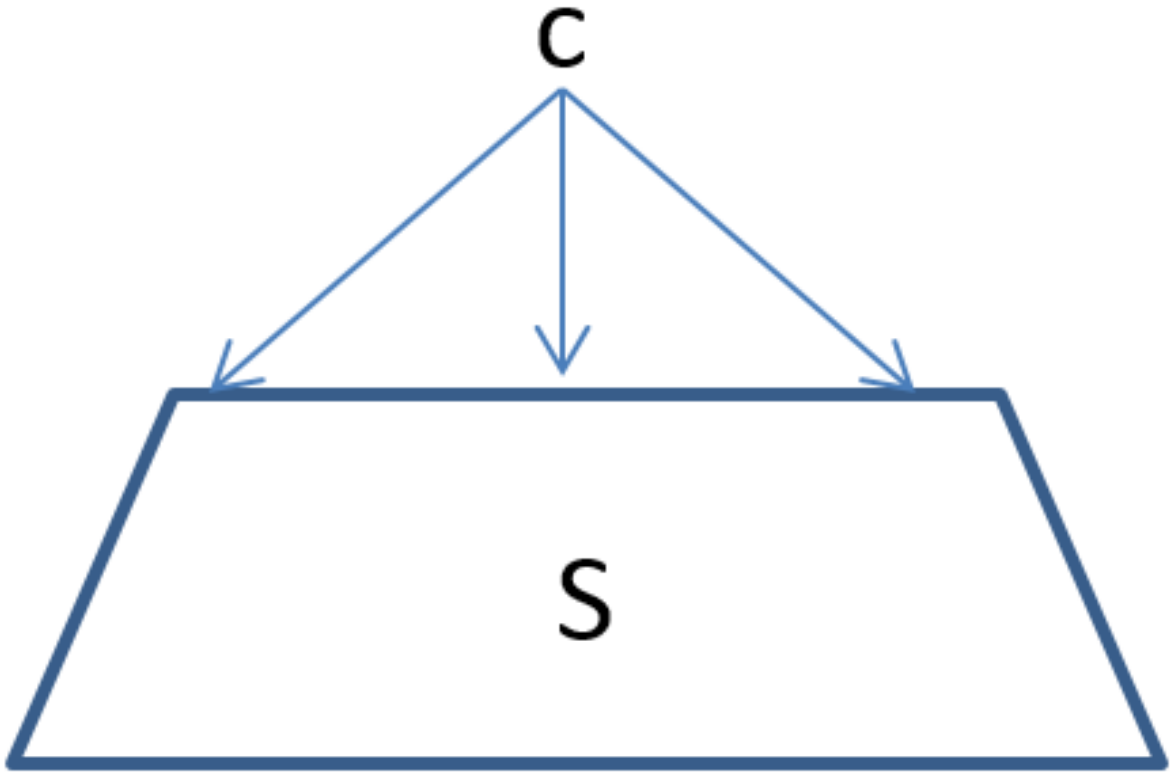
\includegraphics[width=.5\textwidth]{../img/endgame-solving-gadget.png}
      \end{figure}
    \end{frame}

    \begin{frame}{Endgame Solving: Linear Program}
      \begin{equation*}
        \label{lp:endgame-solving}
        \begin{split}
          \max_{v, x}\  f^\top v & \\
          Ex &= e \\
          F^\top v - A^\top x &\le \vect{0} \\
          x &\ge \vect{0}
        \end{split}
      \end{equation*}
    \end{frame}
  }

  \section{CFR-D Decomposition}
  \begin{frame}{CFR-D Decomposition: Gadget Game}
    \begin{figure}[H]
      \centering
      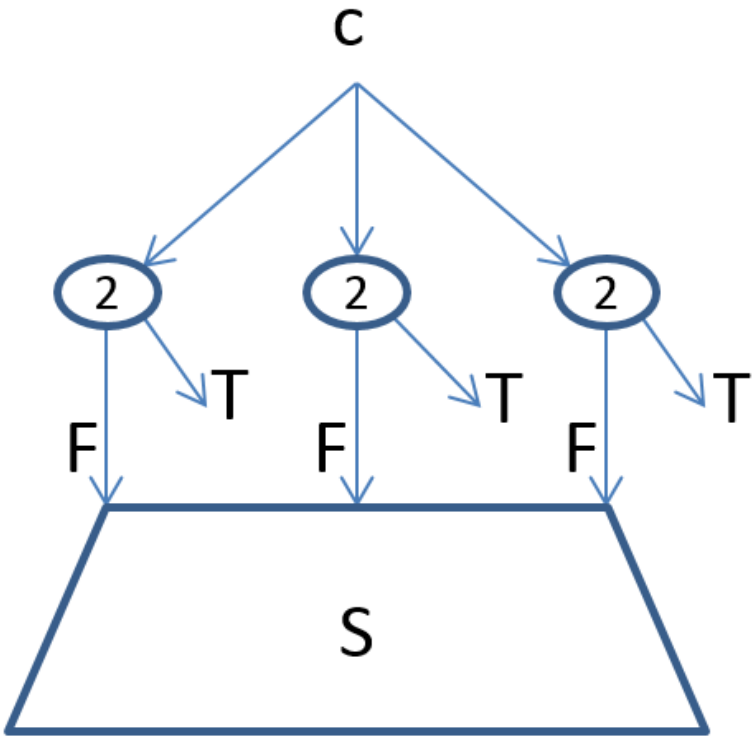
\includegraphics[width=.4\textwidth]{../img/re-solving-game-gadget.png}
    \end{figure}
    \pause

    \begin{itemize}[<+- | alert@+>]
      \item choice of~either to (F)ollow the action into the endgame, or to (T)erminate
      \item utility after the (T)erminal action set to the \emph{counterfactual best-response value}
    \end{itemize}
  \end{frame}

  \begin{frame}{CFR-D Decomposition: Linear Program}
    \begin{equation*}
      \label{lp:cfr-d}
      \begin{split}
        \max_{v, x}\ &0 \\
        \color{red}
        v_I - m &
        \color{red}
        \ge CBV_2^{\sigma_1}(I), \quad I \in \I_2^{R(S)}\\ 
        Ex &= e \\
        F^\top v - A_{\color{red}2}^\top x &\le \vect{0} \\
        x &\ge \vect{0}
      \end{split}
    \end{equation*}
    \pause

    \begin{itemize}[<+- | alert@+>]
      \item $\I_2^{R(S)}$ denotes the root information sets 
      \item $CBV_2^\sigma(I)$ is $2$'s original counterfactual best-response value
    \end{itemize}
  \end{frame}

  \section{Subgame-Margin Maximization}

  \begin{frame}{Subgame-Margin Maximization: Subgame Margin}
    \pause
    \begin{framed}
      Let $\sigma_1$, $\sigma_1'$ be a~pair of~player~$1$'s strategies for subgame~$S$.
      Then a~\textbf{subgame margin} (SM) is
      \[
        SM_1 (\sigma_1, \sigma_1' , S) =
        \min_{I_2 \in \I_2^{R(S)}}
        \left( CBV_2^{\sigma_1} (I_2) - CBV_2^{\sigma_1'} (I_2) \right)
      \]
    \end{framed}
    \pause

    \begin{itemize}[<+- | alert@+>]
      \item ``gap'' between old and new counterfactual best-response values
      \item across all root information sets $I_2 \in \I_2^{R(S)}$
    \end{itemize}
  \end{frame}

  \begin{frame}{Subgame-Margin Maximization: Non-negative SM}
    \begin{framed}
      \begin{Theorem}[\cite{BurchJohansonBowling2014}]
        Given a~strategy~$\sigma_1$, a~subgame~$S$, and a~re-solved subgame strategy~$\sigma_1^S$, let $\sigma_1' = \sigma_{1, [S \leftarrow \sigma_1^S]}$ be the combination of~$\sigma_1$ and~$\sigma_1^S$.
        If $SM_1 (\sigma_1, \sigma_1' , S) \geq 0$, then
        \[
          u_2(\sigma_1', \textrm{CBR}(\sigma_1')) \leq  u_2(\sigma_1, \textrm{CBR}(\sigma_1)).
        \]
      \end{Theorem}
    \end{framed}
    \pause

    Hence, non-negative SM does not allow the opponent to improve.
    \pause

    Moreover, SM is even proportional to the overall improvement$\ldots$
  \end{frame}

  \begin{frame}{Subgame-Margin Maximization: Gain Is Proportional to SM}
    \pause
    \begin{framed}
      \begin{theorem}
        If there is $\sigma_2^* = BR(\sigma_1')$ with $\pi^{<\sigma_1',\sigma_2^*>} (I_2) > 0$ for some $I_2 \in\I_2^{R(S)}$, then the gain in~utilities is proportional to SM:
        \[
          u_1(\sigma_1', CBR(\sigma_1')) - u_1(\sigma_1, CBR(\sigma_1)) \ge \pi_{-2}^{\sigma_1'} (I_2) \cdot SM_1(\sigma_1, \sigma_1', S).
        \]
      \end{theorem}
    \end{framed}
    \pause

    \begin{itemize}[<+- | alert@+>]
       \item ``the probability of~reaching a~subgame'' $\propto \pi_{-2}^{\sigma_1'}(I_2)$
       \item $\uparrow \pi_{-2}^{\sigma_1'}(I_2)$
         \begin{enumerate}[$\Rightarrow$]
           \item $\uparrow$ the bound
           \item $\uparrow$ the probability of~reaching that subgame
         \end{enumerate}
       \item Thus, subgames with larger bounds are likelier to be reached.
    \end{itemize}
  \end{frame}

  \begin{frame}{Subgame-Margin Maximization: Linear Program}
    \begin{equation*}
      \label{lp:max-margin}
      \begin{split}
        \max_{v, x}\ &\textcolor{red}{m} \\
        v_I - m &\ge CBV_2^{\sigma_1}(I), \quad I \in \I_2^{R(S)}\\ 
        Ex &= e \\
        F^\top v - A_2^\top x &\le \vect{0} \\
        x &\ge \vect{0}
      \end{split}
    \end{equation*}
    \pause

    \begin{itemize}[<+- | alert@+>]
      \item $m$ is a~scalar corresponding to the subgame margin
      \item $\approx$ ``gap'' between values $v_I$ and the given constants $CBV_2^\sigma(I)$
      \item \emph{CFR-D Decomposition} only guarantees a~non-negative margin
      \item \emph{Subgame-Margin Maximization} maximizes it
    \end{itemize}
  \end{frame}

  \begin{frame}{Subgame-Margin Maximization: Gadget Game}
    \begin{figure}
      \centering
      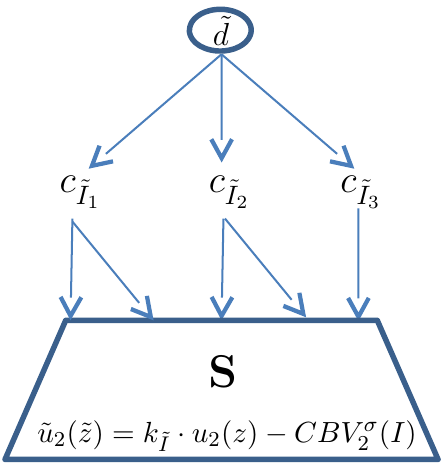
\includegraphics[width=.5\textwidth]{../img/max-margin-gadget.png}
    \end{figure}
    \pause

    Against the original strategy, opponent has a~zero utility at~best.
  \end{frame}

  \begin{frame}{Subgame-Margin Maximization: Experimental Results}
    \begin{figure}[H]
      \centering
      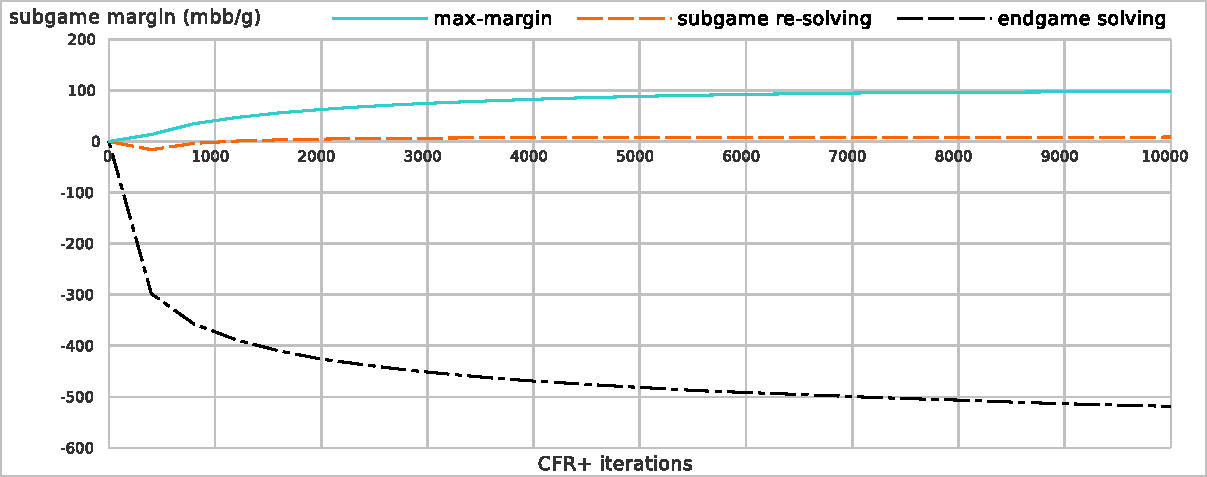
\includegraphics[width=\textwidth]{../img/sm-experiments}
    \end{figure}
    \pause

    \begin{itemize}[<+- | alert@+>]
      \item refinement of~$\approx 2000$ subgames by each method
      \item average margins displayed
      \item max-margin $\to$ the best value, better than subgame re-solving or endgame solving (negative SM!)
    \end{itemize}
  \end{frame}

  \section{Ideas for Future Work}

  \begin{frame}{Margins as a~Vector Linear Program}
    \begin{equation*}
      \label{vlp:max-margins}
      \begin{split}
        \max_{v, x}\ &\textcolor{red}{\vect{m}} \\
        v_I - \vect{m}_{\textcolor{red}{I}} &\ge CBV_2^{\sigma_1}(I), \quad I \in \I_2^{R(S)}\\ 
        Ex &= e \\
        F^\top v - A_2^\top x &\le \vect{0} \\
        x &\ge \vect{0}
      \end{split}
    \end{equation*}

    \pause
    \begin{itemize}[<+- | alert@+>]
      \item $\vect{m}_I := CBV_2^{\sigma_1} (I) - CBV_2^{\sigma_1'} (I)$ corresponds to one specific margin
      \item $\vect{m} := (m_I) _{I\in\I_2^{R(S)}}$ is a~vector of~all such margins
      \item multi-criteria optimization problem
      \item corresponding gadget games?
    \end{itemize}
  \end{frame}

  \begin{frame}[standout]
    \begin{center}
      Thank you!
    \end{center}
  \end{frame}

  \begin{frame}[allowframebreaks]{References}
    \tiny
    \printbibliography[heading=none]
  \end{frame}

\end{document}
